
%%%%%%%%%%%%%%%%%%%%%%%%%%%%%% Sets the document class for the document
% Openany is added to remove the book style of starting every new chapter on an odd page (not needed for reports)
\documentclass[12pt,english,openany,a4paper]{book}

%%%%%%%%%%%%%%%%%%%%%%%%%%%%%% Loading packages that alter the style
\usepackage[]{graphicx}
\usepackage{subcaption}
\usepackage[]{color}
\usepackage{alltt}
\usepackage[T1]{fontenc}
\usepackage[utf8]{inputenc}
\usepackage{makecell}
\setcounter{secnumdepth}{3}
\setcounter{tocdepth}{3}

\usepackage[shortlabels]{enumitem}
% \usepackage{amssymb}
\usepackage{url}
\def\UrlBreaks{\do\/\do-}
\usepackage{ulem}
\usepackage[figuresleft]{rotating}
% \usepackage{xcolor}
% \usepackage{libertine}
% \usepackage{pdfpages}
\usepackage[toc,page]{appendix}
% \usepackage{cite}

% \setlength{\parskip}{\smallskipamount}
\parskip 1.8ex % paragraph spacing
% \setlength{\parindent}{10ex}

% \renewcommand{\baselinestretch}{1.20} % line spacing
\usepackage{multirow}
\usepackage{makecell}
\usepackage{siunitx}
\sisetup{
   detect-mode,
   detect-family,
   detect-inline-family=math,
}

\usepackage{mathptmx}


% Set page margins
\usepackage[top=100pt,bottom=100pt,left=68pt,right=66pt]{geometry}

% Package used for placeholder text
% \usepackage{lipsum}

% Use to cross cite in document
% \usepackage{notoccite}

% Prevents LaTeX from filling out a page to the bottom
\raggedbottom

% Adding both languages
\usepackage[english]{babel}

% All page numbers positioned at the bottom of the page
\usepackage{fancyhdr}
\fancyhf{} % clear all header and footers
\fancyfoot[C]{\thepage}
\renewcommand{\headrulewidth}{0pt} % remove the header rule
\pagestyle{fancy}

% Changes the style of chapter headings
\usepackage{titlesec}
\titleformat{\chapter}
   {\normalfont\LARGE\bfseries}{\thechapter.}{1em}{}
% Change distance between chapter header and text
\titlespacing{\chapter}{0pt}{50pt}{2\baselineskip}

% Adds table captions above the table per default
% \usepackage{float}
% \floatstyle{plaintop}
% \restylefloat{table}

% Adds space between caption and table
\usepackage[tableposition=top]{caption}

% Modern implementation of the bookmarks managing is used without .out file. The bookmarks are updated earlier, thus in most cases only one LaTeX run is needed.
\usepackage{bookmark}

% Adds hyperlinks to references and ToC
\usepackage{hyperref}
\usepackage{cleveref}
\hypersetup{hidelinks,linkcolor = black} % Changes the link color to black and hides the hideous red border that usually is created
% \hypersetup{linkcolor = black}

% If multiple images are to be added, a folder (path) with all the images can be added here 
\graphicspath{ {Figures/} }

% Separates the first part of the report/thesis in Roman numerals
\frontmatter
\usepackage[sort&compress,numbers,comma,square]{natbib} %for references

\setlength{\bibsep}{1.8ex plus 0.3ex}
\renewcommand{\bibname}{References}
%\renewcommand{\bibfont}{\normalfont\scriptsize}
\makeatletter
\renewcommand\@biblabel[1]{[#1]}
\makeatother
\newcommand\blfootnote[1]{%
  \begingroup
  \renewcommand\thefootnote{}\footnote{#1}%
  \addtocounter{footnote}{-1}%
  \endgroup
}
\linespread{1}


\titleformat{\chapter}{\normalfont\LARGE\bfseries}{\thechapter}{1em}{}
\titlespacing{\chapter}{0pt}{3.5ex plus 1ex minus .2ex}{2.3ex plus .2ex}

\makeatletter
\renewcommand*\l@figure{\@dottedtocline{1}{0em}{2.3em}}% Default: 1.5em/2.3em
\let\l@table\l@figure
\makeatother

\renewcommand{\bibname}{References}


%%%%%%%%%%%%%%%%%%%%%%%%%%%%%% Starts the document
\begin{document}

%%% Selects the language to be used for the first couple of pages
\selectlanguage{english}

%%%%% Adds the title page
\begin{titlepage}
  \vspace{3 cm}
  \begin{center}
  \large{\textbf{Detection of roads networks in mid-resolution satellite image}}\bigskip \\
  
  \vspace{3mm}
  \vfill
  BTP  Report \\
  by \bigskip \\
  \textbf{Nautatava Navlakha\\(Roll Number: 160040007)}
  \vfill
  \textbf{Supervisor}\\
  Prof. Gopal Patil\\
\vfill  \begin{figure}[h]
  \includegraphics[width=50mm]{logo_iitb}
  \centering
  \end{figure}
  \vfill
  \large
  
Civil Engineering\\
Indian Institute of Technology Bombay\\
May, 2020
\end{center}
\vfill % Fill the rest of the page with whitespace
\end{titlepage}




\pagenumbering{roman}

% \clearpage
% \thispagestyle{empty}
% \phantom{a}
% \vfill
% \begin{center}{\large \textit{This page has been intentionally left blank}}\end{center}
% \vfill

% \newpage
% \chapter*{Abstract}
The economy is moving towards automation. Roads are an essential factor in growth, development, and providing services. Though documented extensively in papers, the detection of small roads in mid-resolution satellites is still a problem. The work here sheds light on combining the low-level computer vision problem of super-resolution with the high-level computer vision problem of road-detection. We investigate the behavior when we first enhancing the image resolution before directly apply road-detection. We try to identify the small roads from a mid-resolution satellite image, which are otherwise skipped by the model prediction by combining the two different levels of computer vision problems.

The model uses Convolutional Neural Networks supported by ResNet architecture. It also uses encoder-decoder and dilated convolutions to segment the image to identify roads and take the spatial context into account. The method described here allows us to improve the capability of any model to now detect finer roads.


% \clearpage
% \thispagestyle{empty}
% \phantom{a}
% \vfill
% \begin{center}{\large \textit{This page has been intentionally left blank}}\end{center}
% \vfill

% \begin{center}
{\LARGE \textbf{ Declaration}}
\end{center}
I hereby declare that the matter contained in this report titled  \textbf{``Low Temperature Atomic Layer Deposition of {SiO2}"} is an authentic record of research work carried out by me at the \textbf{Devices and Interfaces Lab, Department of Energy Science and Engineering, Indian Institute of Technology Bombay, Mumbai} under the supervision of \textbf{ Prof. Shaibal K. Sarkar}, as part of the \textbf{M. Sc. - Ph. D. Dual Degree Programme} from \textbf{June 2019} to \textbf{November 2019}.\bigskip\\
I declare that this written submission represents my ideas in my own words and where others' ideas or words have been included, I have adequately cited and referenced the original sources. I declare that I have properly and accurately acknowledged all sources used in the production of this report. I also declare that I have adhered to all principles of academic honesty and integrity and have not misrepresented or fabricated or falsified any idea/data/fact/source in my submission. I understand that any violation of the above will be a cause for disciplinary action by the Institute and can also evoke penal action from the sources which have thus not been properly cited or from whom proper permission has not been taken when needed. Any oversight due to error of judgement is regretted.
\vspace{3 cm}

\begin{tabular}{p{80mm}  p{80mm}}
     Date: 20$^{\rm th}$ November 2019 &\makecell[r]{Aditya Chalishazar\\ Place: Mumbai} 
\end{tabular}


% \clearpage
% \thispagestyle{empty}
% \phantom{a}
% \vfill
% \begin{center}{\large \textit{This page has been intentionally left blank}}\end{center}
% \vfill

% \begin{center}
{\LARGE \textbf{ Certificate}}
\end{center}
This is to certify that the matter contained in this report titled \textbf{``Low Temperature Atomic Layer Deposition of {SiO2}"}  is the result of the work performed by \textbf{ Mr. Aditya Chalishazar} at the \textbf{Devices and Interfaces Laboratory, Department of Energy Science and Engineering, Indian Institute of Technology Bombay, Mumbai} under my supervision, as part of the \textbf{M. Sc. - Ph. D. Dual Degree Programme} from \textbf{June 2019} to \textbf{November 2019}.
\vspace{3 cm}

\begin{tabular}{p{80mm}  p{80mm}}
     Date: 20$^{\rm th}$ November 2019 &\makecell[r]{Prof. Shaibal K. Sarkar\\ Place: Mumbai} 
\end{tabular}


% \clearpage
% \thispagestyle{empty}
% \phantom{a}
% \vfill
% \begin{center}{\large \textit{This page has been intentionally left blank}}\end{center}
% \vfill
% \begin{center}
    \textbf{\LARGE Acknowledgement}
\end{center}
\noindent
The success of any endeavour is the contributions of several individuals.\smallskip\\

\noindent
I would like to express my sincere gratitude to my supervisor Prof. Shaibal K. Sarkar, for the opportunity to work under his guidance and his invaluable comments and suggestions regarding my work.\smallskip\\

\noindent
I owe a deep sense of gratitude to Mr. Bireswar Mandol for his continuous support in guiding my work and explaining the nuances of research work.\smallskip\\

\noindent
I extend my sincere thanks to Prof. Rangan Banerjee, the Head, Department of Energy Science and Engineering for this opportunity to be part of the M. Sc. - Ph. D. programme.\smallskip\\

\noindent
I extend my gratitude to Prof. Pratibha Sharma, Faculty Advisor for her support and suggestions.\smallskip\\

\noindent
I extend my gratitude to all other members of the laboratory: Dr. Chetan Singh, Dr. Neha Mahuli, Dr.~Anand Selvin S., Dr. Arpan Dhara, Dr. Ansuman Halder, Dr. Dayanand Sutar, Dr. Arpita Sarkar, Ms. Roja Singh, Ms. Vidya Raj, Ms. Sudeshna Ghosh, Mr. Alok Tiwari, Mr. Gaurav Bansode, Mr. Vikas Munya, Ms. Raj Rani, Ms. Shreya Sharma, Ms. Nisha Sarda, Mr. Arya Vikram for their guidance and support.\smallskip\\

\noindent
I am also grateful for the help and support of Ms. Prerna Goradia and Ms. Geetika Bajaj for their help in sample characterisation.\smallskip\\  

\noindent
I am extremely grateful for the continuous encouragement and support of my family, teachers and my friends.\smallskip\\

\noindent
I am grateful for the abundant blessings of the Almighty in every endeavor I have undertaken.

\tableofcontents
\newpage

\listoffigures
\addcontentsline{toc}{chapter}{\numberline{}List of Figures}

\newpage
\listoftables
\addcontentsline{toc}{chapter}{\numberline{}List of Tables}

\clearpage
%\includepdf[pages={10}, pagecommand={}]{external.pdf}
%\chapter{Nomenclature}\label{tab:nomenclature}

\section{Data related}
\textbf{OSM}:  Open Street Map \\
\textbf{RGB}:  Red, Green, Blue \\
\textbf{HR}:   High Resolution \\

\section{Machine Learning related}
\textbf{AI}:   Artificial Intelligence \\
\textbf{ML}:   Machine Learning \\
\textbf{PSNR}: Peak Signal to Noise Ratio \\
\textbf{BP}:   Back Propagation \\
\textbf{SVM}:  Support Vector Machine \\
\textbf{ReLU}: Rectified Linear Unit \\
\textbf{ANN}:  Artificial Neural Network \\
\textbf{CNN}:  Convolutional Neural Network \\
\textbf{DCNN}: Deep Convolutional Neural Network \\
\textbf{SR}:   Super Resolution \\
\textbf{EDSR}: Enhanced Deep Super Resolution \\
\textbf{VDSR}: Very Deep Super Resolution \\
\textbf{FCN}:  Fully Connected Network \\

\section{Hardware related}
\textbf{RAM}:  Random Access Memory \\
\textbf{MSI}:  Multispectral Instrument \\
\textbf{MB~/~GB}:   MegaByte~/~GigaByte \\
\textbf{GPS}:  Global Positing Systems \\ 
\textbf{GPU}:  Graphics Processing Unit \\
\textbf{TPU}:  Tensor Processing Unit \\


\pagenumbering{arabic}

%%%%%%%%%%%%%%%%%%%%%%%%%%%%%%%%%%%%%%%%%%%%%%%%%%%%%%%%%%%%%%%%%%%%%%%%%%%%%%%%%%%%%%%%%%%%
%%%%%%%%%%%%%%%%%%%%%%%%%%%%%%%%%%%%%%%%%%%%%%%%%%%%%%%%%%%%%%%%%%%%%%%%%%%%%%%%%%%%%%%%%%%%
%%%%% Text body starts here!
\mainmatter
% TODO: maitain consistency for super-resolution and road-detection. See caps and smalls too!
% TODO: How to add Nomenclature. Do I need it for aliases?
% TODO: Checkout capitalisation for references, eg: table, figure, chapter 4.xx
\chapter{Nomenclature}\label{tab:nomenclature}

\section{Data related}
\textbf{OSM}:  Open Street Map \\
\textbf{RGB}:  Red, Green, Blue \\
\textbf{HR}:   High Resolution \\

\section{Machine Learning related}
\textbf{AI}:   Artificial Intelligence \\
\textbf{ML}:   Machine Learning \\
\textbf{PSNR}: Peak Signal to Noise Ratio \\
\textbf{BP}:   Back Propagation \\
\textbf{SVM}:  Support Vector Machine \\
\textbf{ReLU}: Rectified Linear Unit \\
\textbf{ANN}:  Artificial Neural Network \\
\textbf{CNN}:  Convolutional Neural Network \\
\textbf{DCNN}: Deep Convolutional Neural Network \\
\textbf{SR}:   Super Resolution \\
\textbf{EDSR}: Enhanced Deep Super Resolution \\
\textbf{VDSR}: Very Deep Super Resolution \\
\textbf{FCN}:  Fully Connected Network \\

\section{Hardware related}
\textbf{RAM}:  Random Access Memory \\
\textbf{MSI}:  Multispectral Instrument \\
\textbf{MB~/~GB}:   MegaByte~/~GigaByte \\
\textbf{GPS}:  Global Positing Systems \\ 
\textbf{GPU}:  Graphics Processing Unit \\
\textbf{TPU}:  Tensor Processing Unit \\

\chapter{Introduction}\label{chapt:intro}

Monitoring roads is an essential element in urban planning. Almost every city is developed around centers with adequate transportation facilities. They provide infrastructural support to both the agricultural and industrial sectors of every country. Given its uses in disaster management, transportation of facilities, social interaction, it is historically proven that everything can efficiently work out if we have a proper mapped site. Mapping the roads, thus, is of utmost importance.

Historically, roads were mapped manually using approximate measures, mostly for short distances, and to help religious pilgrims navigate. With the development of automobiles, maps soon became more extensive and kept in the form of books~\cite{firstMapBooks}. These were handwritten until digital maps could be produced. With the help of Global Positing Systems~(GPS) navigation, maps started becoming digital and electronic versions were kept. These electronic versions had many advantages over their paper counterparts. With digital versions, the limitations of paper: wearability, tendency to be lost or damaged easily, is no longer a pressing issue. 

Though the digital versions could now be replicated easily by printers or by transferring files to other supported devices, taking GPS enabled devices to mark roads is both inefficient and costly. Some roads are inaccessible due to various factors. To combat the individual mapping of roads, some open crowdsourcing platforms like \href{https://www.openstreetmap.org/}{OpenStreetMap~(OSM)} help people continue researching by using their data. This successfully reduced the redundant work, but there is no way to check if the data is correct. Almost always, human errors reduce the quality of data. Millions of kilometers of roads are still left to be digitized to be used for any activity~\cite{MapsDoneOSM}. As previous road data might have changed, completing the mapping of the remaining roads still does not guarantee us the latest report.

The computer is one piece of technology which makes our work a lot simpler. With the advent of techniques such as Machine Learning, identifying patterns to solve certain kinds of problems has become a lot easier. This work is an attempt to use image segmentation based on computer vision techniques to detect roads in satellite images. This will help us in reducing the manual workforce to a large extent. While road detection has been extensively documented in research papers, these papers mostly focus on identifying roads while the camera is on the road. While this has it's own uses in navigation, but using these techniques for surveying is not feasible as one will have to drive all the way, resulting in highly inefficient surveying. Some papers have tried to overcome this problem by high-resolution satellite images, but high-resolution images are quite expensive and have to be bought commercially. Another widespread problem these satellite images face is radiometric distortion. Roads of asphalt, sometimes turn from dark grey into bright white due to some reflection affecting satellite sensors. This is seen clearly is \cref{fig:sat_img_radiometric_distortion}~\cite{GF2-imageCaseStudy}. 

\begin{figure}[h!]
  \centering
  \begin{subfigure}{0.48\textwidth}
    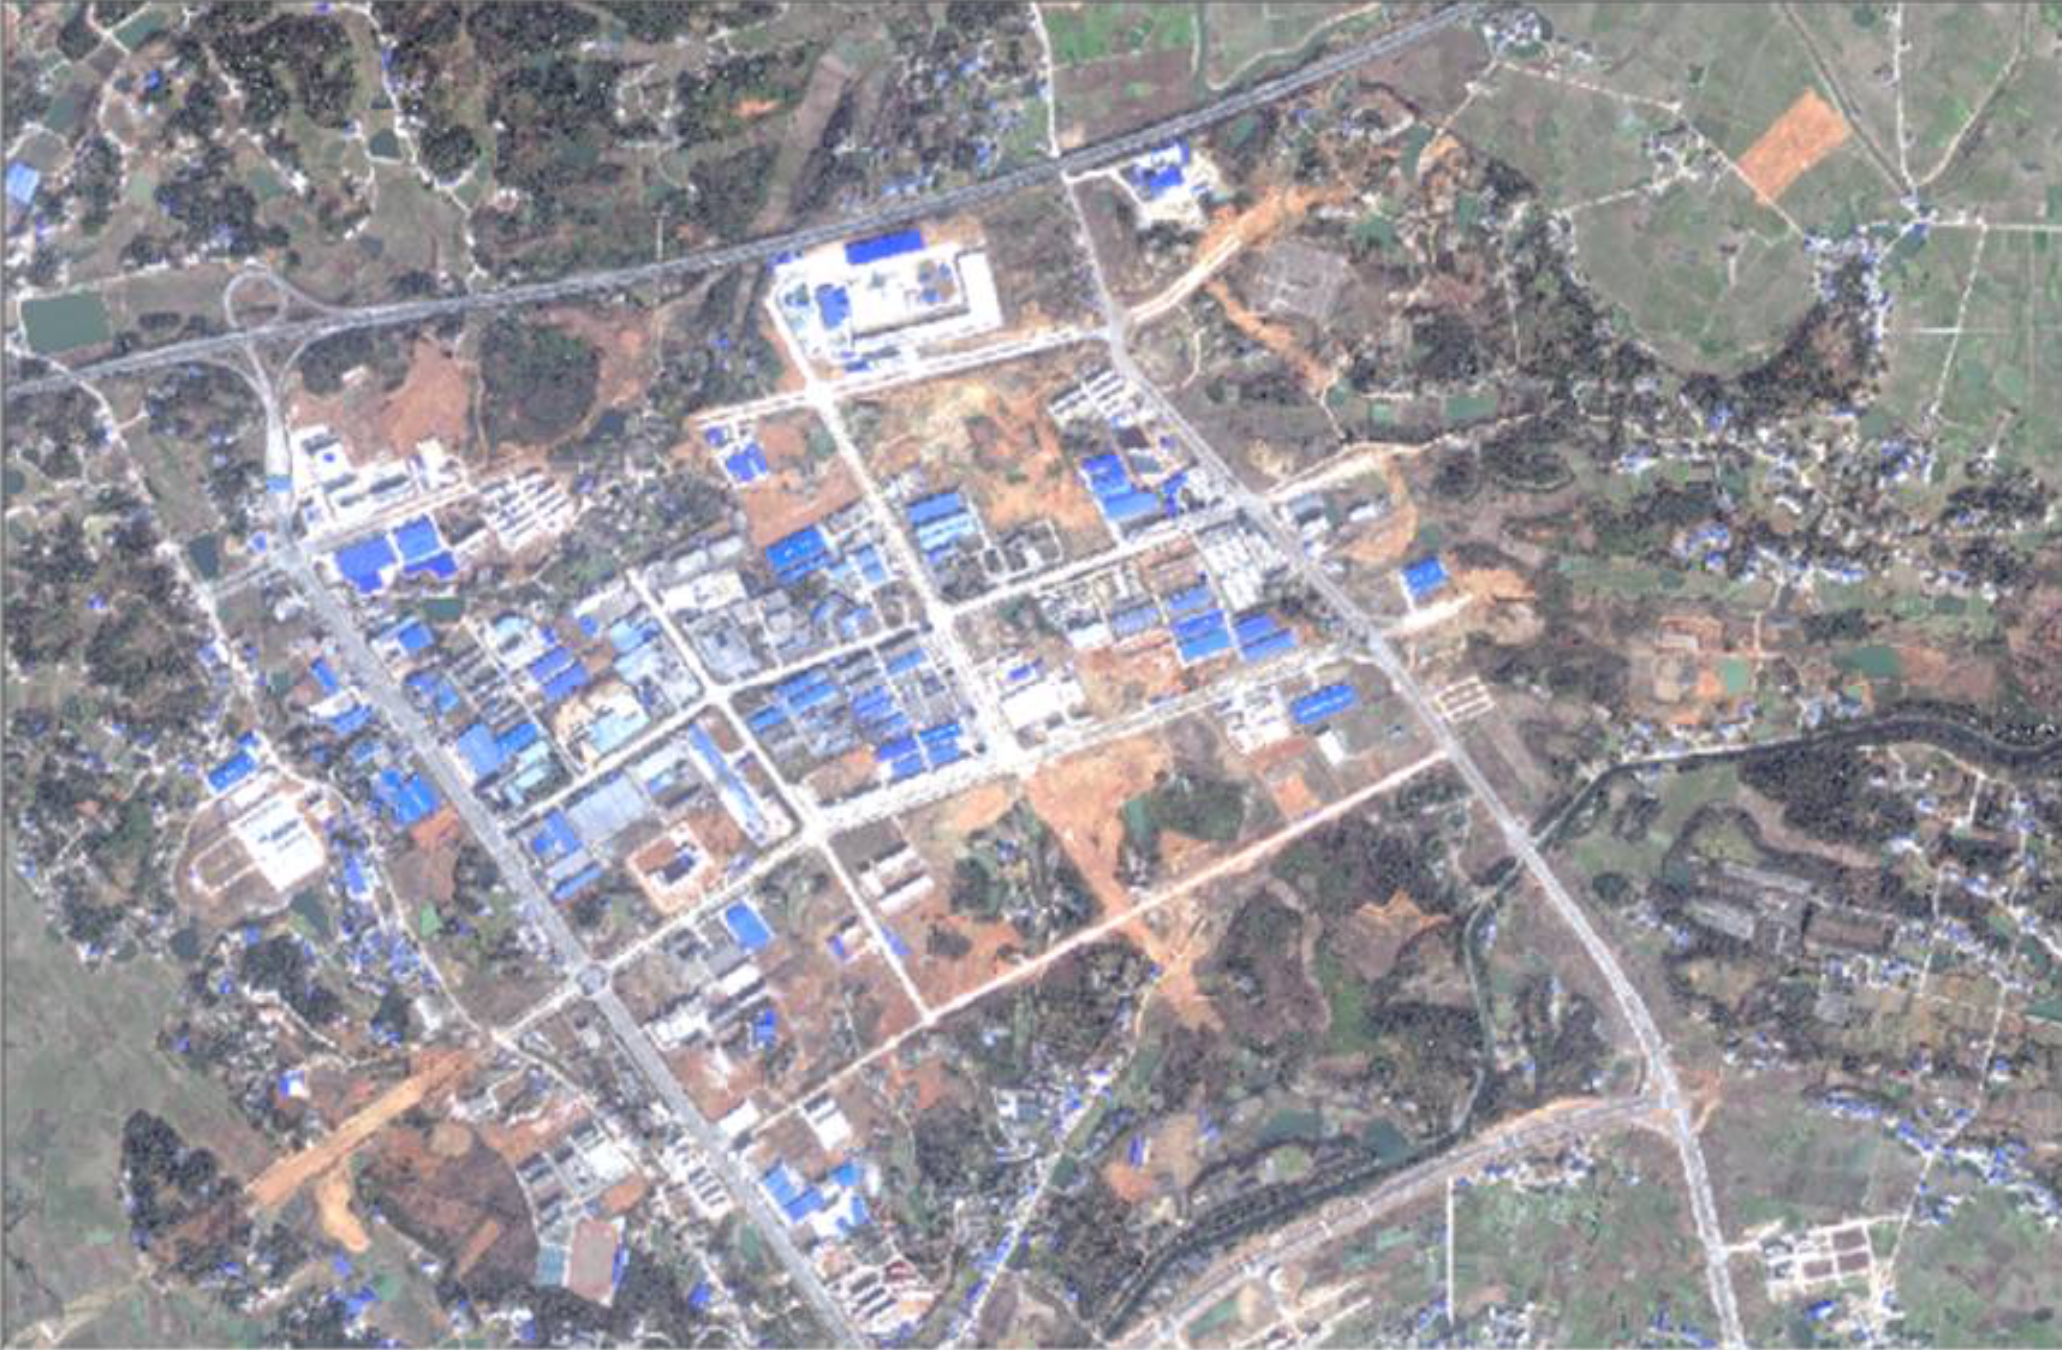
\includegraphics[width=\textwidth]{sat_img_GF2_radiometric_distortion}
    \caption{}
  \end{subfigure}~
  \begin{subfigure}{0.48\textwidth}
    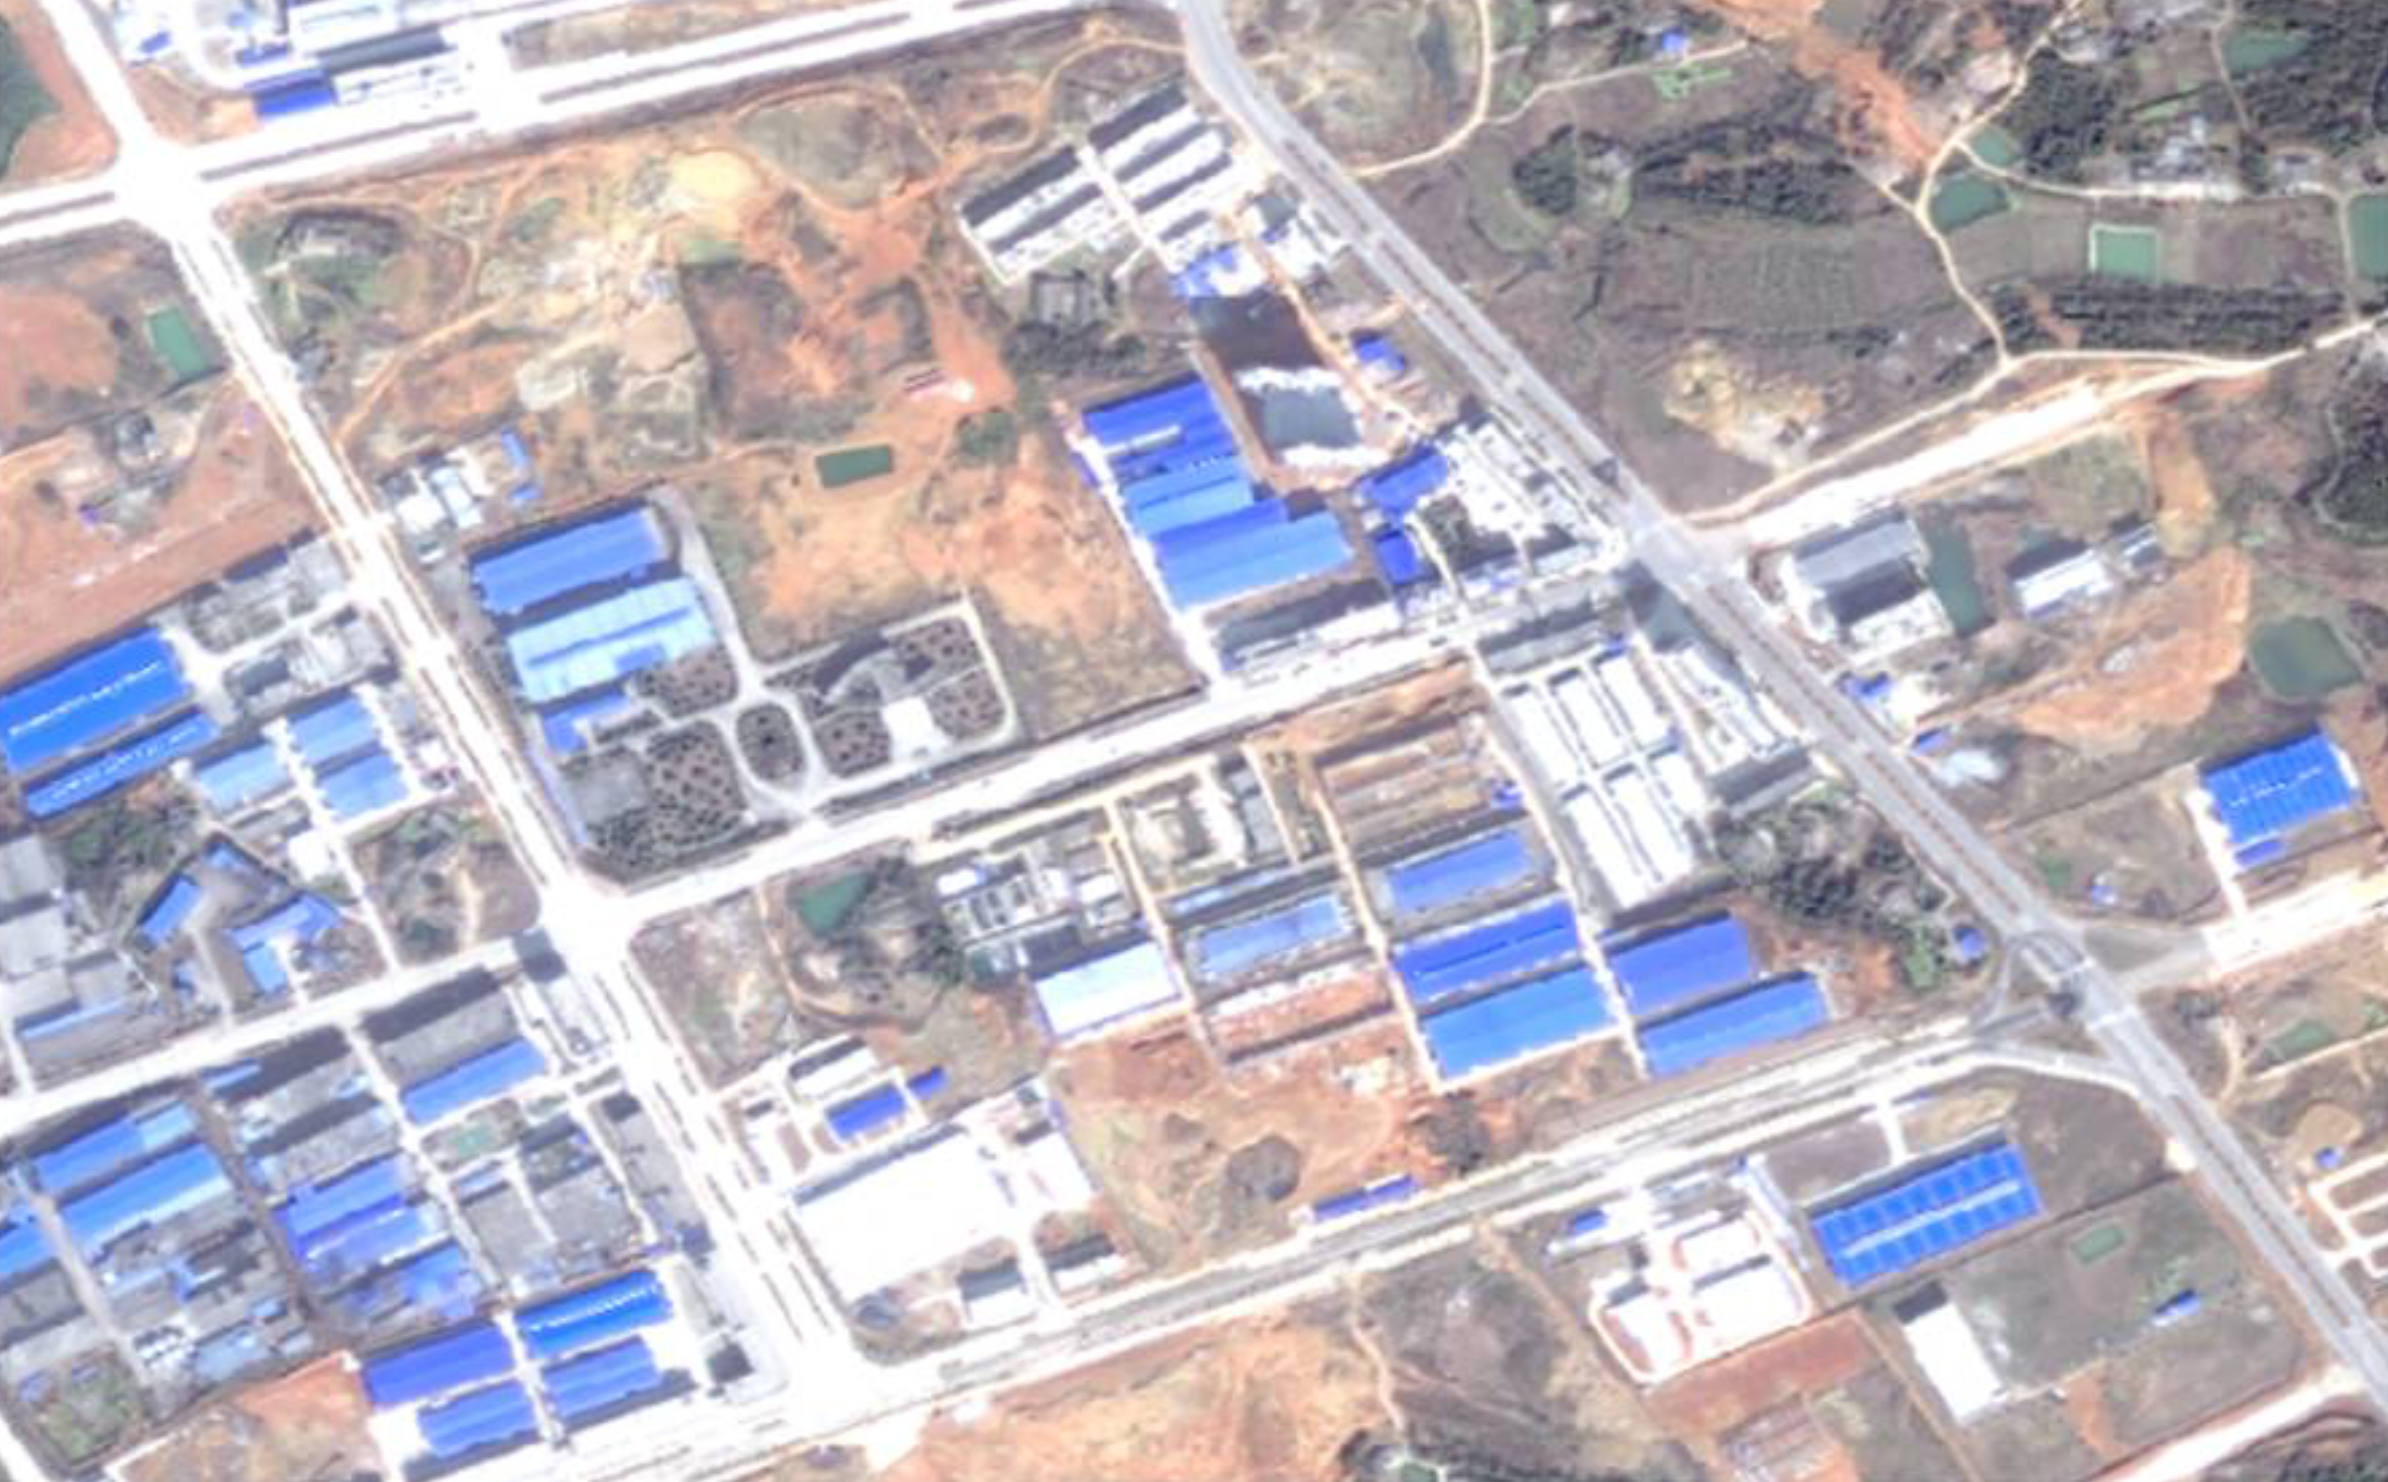
\includegraphics[width=\textwidth]{sat_img_zoomed_GF2_radiometric_distrotion}
    \caption{}
  \end{subfigure}
  \caption[Optical distortion clearly visible on roads]{Optical distortion clearly visible on roads. \textbf{(a)}~Radiometric distortion in image from GF2 satellite. \textbf{(b)}~Zoomed image of (a). Taken from~\cite{GF2-imageCaseStudy}.}
  \label{fig:sat_img_radiometric_distortion}
\end{figure}

We will be using mid-resolution satellite images as they can be used for large scale surveys to tackle distortion and reduce the cost. The identification of roads on mid-resolution~(>~5~m) satellite data is difficult and often has low accuracy. A typical two-lane road has a width of around 7~m, and this road will have a width of hardly a pixel in our satellite image. This work is an effort to use image segmentation techniques in the area of remote sensing to detect roads in mid-resolution satellite images.

When applying existing road-detection algorithms to mid-resolution satellite images, the algorithm is able to predict the location of wide roads successfully. What remains an issue are the roads which occupy about 1~pixel in the image. Two reasons can be thought upon for this issue. One hypothesis is that our algorithm is unable to classify the pixel-level road properly. However, it correctly classified the roads which have, say 4~pixels. A filter, if taken appropriate steps, cannot be biased again these roads. Hence, the only possible option is that our filters are unable to detect any edge in the roads occupying just a pixel. The most intuitive way to counter this problem is to break down an individual pixel into $x$ different pixels. This is the same problem that super-resolution promises to solve. Hence, in this work, we try to detect roads using a model consisting of super-resolution and road-detection as its subcomponents.


RGB images from satellite \href{https://sentinel.esa.int/web/sentinel/missions/sentinel-2}{Sentinel-2A} is used in this work-report. \Cref{tab:sentinel-resolution} lists the detailed parameters of the satellite. Band 2 (Blue), 3 (Green), and 4 (Red) are stacked together to get a 3-channel RGB image. As seen in the specifications, the spacial resolution of the final image is 10~m. The task is to increase the accuracy of the existing road-detection algorithm.

\begin{table}[h!]
  \centering
  \begin{tabular}{ |c|c|c| }
    \hline
    Spatial resolution~(m) & Band number & Central wavelength~(nm) \\
    \hline
    10&2&492.4 \\
    10&3&559.8 \\
    10&4&664.6 \\
    10&8&832.8 \\
    20&5&704.1 \\
    20&6&740.5 \\
    20&7&782.8 \\
    20&8a&864.7 \\
    20&11&1613.7 \\
    20&12&2202.4 \\
    60&1&442.7 \\
    60&9&945.1 \\
    60&10&1373.5 \\
    \hline
  \end{tabular}
  \caption[Wavelengths and bandwidths of the three spatial resolutions of the MSI instruments]{Wavelengths and bandwidths of the three spatial resolutions of the MSI instruments~\cite{sentinelSpecifications}.}
  \label{tab:sentinel-resolution}
\end{table}

By combining the three bands from the raw satellite image, the resulting image size is of the order of 400~MB for one mid-sized city. At first, this may not seem significant in comparison with some of the media files. Yet, handling files of this size in DCNN is a severe issue. Processing large files might be possible for massive supercomputers; however a general workstation has Random Access Memory~(RAM) anywhere from 128 to 256~GBs of RAM, while personal computers range from 8~GB to 32~GBs of RAM. Thus, this image must be divided into several parts so that our algorithms work on a readily available device.

Our input image does not have a sufficiently high resolution to identify small roads. To deal with this problem of pixelization, we will be using two types of models. This setup is shown in \cref{fig:model_complete_without_labels}. Unless specifically mentioned, a model means a combined setup using super-resolution and road-detection models. Data from the input layer goes to the super-resolution model, which is consequently passed to the road-detection model. The final output consists of the predicted road network in the image.

\begin{figure}[h!]
  \centering
  \includegraphics[width=\textwidth]{model_complete_without_labels}
  \caption{Complete setup: Combination of super-resolution and road-detection models.}
  \label{fig:model_complete_without_labels}
\end{figure}

\chapter{Problem definition and background}\label{chapt:problem}
Road digitalization is an expensive operation. Research is being done to identify roads automatically using Artificial Intelligence with the different types of images. High-resolution satellite images are expensive to get, and covering an entire state or country is a nightmare. On the other hand, mid-resolution satellite images can be obtained for free, but the identification of roads on mid-resolution~(>~5~m) satellite data is difficult and often has low accuracy. This work tries to detect the smaller roads~(with 1 or 2 lanes), which are often missed out.

We will be using RGB images from satellite Sentinel-2A. Detailed parameters of the satellite are given in Table~\ref{tab:sentinel-resolution}. Band 2 (Blue), 3 (Green), and 4 (Red) are stacked together to get a 3-channel RGB image. As seen in the specifications, the spacial resolution of the final image is 10~m. The task is to increase the accuracy of the existing road-detection algorithm.

\begin{table}[h!]
  \centering
  \begin{tabular}{ |c|c|c| }
    \hline
    Spatial Resolution~(m) & Band Number & Central Wavelength~(nm) \\
    \hline
    10&2&492.4 \\
    10&3&559.8 \\
    10&4&664.6 \\
    10&8&832.8 \\
    20&5&704.1 \\
    20&6&740.5 \\
    20&7&782.8 \\
    20&8a&864.7 \\
    20&11&1613.7 \\
    20&12&2202.4 \\
    60&1&442.7 \\
    60&9&945.1 \\
    60&10&1373.5 \\
    \hline
  \end{tabular}
  \caption[Wavelengths and Bandwidths of the three Spatial Resolutions of the MSI instruments]{Wavelengths and Bandwidths of the three Spatial Resolutions of the MSI instruments~\cite{sentinelSpecifications}}
  \label{tab:sentinel-resolution}
\end{table}

By combining the three bands from the raw satellite image, the resulting image size is of the order of 400~MB for one mid-sized city. At first, this may not seem significant in comparison with some of the media files. However, handling files of this size in DCNN is a severe issue. 
% Let us see the specifications needed by a computer to handle this image in 1 go:
% TODO: Calculations showing 400MB in DCNN

This might be possible for massive supercomputers, but a general workstation has Random Access Memory~(RAM) anywhere from 128 to 256~GBs of RAM, while personal computers range from 8~GB to 32~GBs of RAM. Thus, this image must be divided into several parts so that our algorithms work on a readily available device.

Our input image does not have a sufficiently high resolution to identify small roads. To deal with this problem of pixelization, we will be using two types of models. This setup is shown in Figure~\ref{fig:model_complete_without_labels}. Unless specifically mentioned, a model means a combined setup using super-resolution and road-detection models. Data from the input layer goes to the super-resolution model, which is consequently passed to the road-detection model. The final output consists of the predicted road network in the image.

\begin{figure}[h!]
  \centering
  \includegraphics[width=\textwidth]{model_complete_without_labels}
  \caption{Complete setup: Combination of Super-resolution and road-detection models.}
  \label{fig:model_complete_without_labels}
\end{figure}


\chapter{Previous Work}\label{chapt:previous}
[\textit{The idea of using satellite data has been researched within many communities. Several automated and semi-automated ways are proposed to tackle the problem of detecting roads. These ways are quite different due to different strategies and aglorithms used by them. The different strategies come into picture to takle the various challenged like noisy data, occlusions, distortion and complex backgrounds which appears in images.}]

\section{Road detection}
The journey to identify roads digitally started with the topic of reducing the cost and increasing produtivity. One of the first road detection algorithms were static methods and focused on color and geometry of roads. This was quite unreliable as shadows on roads had a similar color range, this resulted in many errors and discontinuities \cite{Detecting_interections_using_color,Detecting_roads_using_color}. Another disadvantage was the need of high resolution images (Almost 0.2~m-0.5~m) which is hard to get. The idea was then improvised to include texture cues for road detection \cite{using_texture_for_road_detection,baumgartner1999automatic}. The accuracy was indeed better but need to very high resolution image still remained a problem. With the Machine learning techniques, the pixel-level classification started to give improved performance \cite{road_detection_using_neural_nets_SVM,road_detection_using_env_learning,road_detection_using_SVM_online_learning}. \par

The SVM methods have a good generalization ability, and thus widely used in object detection from a given image. They are, at most times, more accurate and give consistent robust results than other classification techniques such as K-nearest neighbor. But, the estimation of kernel functions and the choice of the dimensional space and training samples give a hard time. % \cite{Yager and Sowmya (2003) and Melgani and Bruzzone (2004)}
exploited the SVM classifier by using edge-based features such as gradient, intensity, edge length and classified objects in a high resolution image. SVM approaches are well suited for multispectral data where we have adequate number of vectors to classify objects % \cite{Simler (2011}
. \par

In 2003, Tu-Ko presented a robust approach, in which a back-propogation(BP) neural network was trained with the spectral and edge information to find the road centerline. Although errors prop in, the model was still useful as a whole. Disadvantages of BP neural network include slow convergence speed, need of a large training data set, inability to find global minima and risks with over-fitting. Since then many types of neural networks like fuzzy neural network \cite{mokhtarzade2008automatic}, and convolutional Neural Networks(CNN) have been used to capture the spacial contexts of road networks, giving much better accuracies on fewer resources. \par

With the developments of GPUs and the progress of ResNet architectures, even Deep Convolutional Neural Networks(DCNN) have been researched and changed the way road extraction works. The recent developments with encoder-decoders, dilations and fuzzy logics have inspired state-of-the-art algorithms like UNet, SegNet, LinkNet, and it's further improvements like D-LinkNet and AD-LinkNet. Moreover competitions pitch in the researchers by providing them with precise dataset and motivating them to thrive and excel in the world race. \par


\section{Super-resolution}
Many models have proposed methods to obtain super-resolution image from a give image. Most of the techniques use bicubic upsampling of image as an input to the proposed neural network model. However, this was inefficient as a significant part of memory is required for performing bicuic upsampling. The authors of % \cite{EDSR} 
additionally questioned the architectural optimality used in the existing networks. Though neural networks provides significantly improved performance in terms of peak signal-to- noise ratio (PSNR) in the SR problem, it is also proved to be quite sensitive to minor architectural changes and The outputs differs in performance with different training techniques. The authors further proposed an enhanced deep super-resolution network (EDSR) with performance exceeding the past state-of-the-art super-resolution models. This was achieved by carefully designing model architecture using sophisticated optimization methods in training the neural networks. \par

Secondly, the authors noticed that most existing models treat super- resolution of different scale factors as an independent problem. There's no consideration of learning the mutual realtionship between different scales. With effprts such as development of VSDR, this realtionship is proved to be not only feasible but is also shown to be much more accurate than the single scale models at the cost of heavier computation time and memory utilization. The further work was restricted by lack of ability to use very deep neural networks. \par

With the break-through changes brought by concepts of skip-connects and residual blocks, it was proved to train the early difficult deep neural networks. SRNet solved encorporated the ResNet architecture and solved the problem of high memory utilization. Because ResNet architecture was proposed to solve higher-level computer vision problems such as image classification and detection, it's use directly for a low-level problem like computer vision can be optimized. \par

EDSR propses using a modified type of residual block to remove the redundant elements and optimize the performance of the model. Secondly, a new architecture is used with fewer parameters but showing comparable performance. The Figure~\ref{fig:compare_SR} shows the comparison between different SR algorithms.

\begin{figure}
  \centering
  \includegraphics[width=\textwidth]{compare_SR}
  \caption[Comparison of different Super-resolution models.]{Comparison of different Super-resolution models. HR is raw high resolution image taken. Adapted from \cite{EDSR}}
  \label{fig:compare_SR}
\end{figure}

\chapter{Literature review}\label{chapt:lit}
\section{Convolutional Neural Networks~(CNN)}
\textit{A CNN is a type of Artificial Neural Network~(ANN) where convolutional blocks are used instead of basic 1-D multilayer perceptrons}

For understanding CNN, we need to see what an Artificial Neural Network~(ANN) is. ANN is a system of interconnected neurons used to model complex functions for classification and regression. Any model is made up of at least three layers: An input layer, one or more hidden layers, and an output layer. The most basic ANN model consists of multilayer perceptrons. \Cref{subsection:types_of_layers} shows different types of layers that can be used for a convolutional neural network. Several nonlinear activation functions such as rectified linear unit (ReLU)or sigmoid, or even custom functions can be applied at any point on the layers to produce activation maps. These activation maps finally help us in classification or segmentation.

\subsection{Types of layers}
\label{subsection:types_of_layers}
The general structure of any convolutional neural network can be categorized as follows:
\begin{enumerate}[(a)]
    \item \textbf{Input layer}:
        The input layer is the input of any neural network. The input of computer vision problems is usually an image that is basically a matrix of numbers stacked multiple times~(channels). An RGB image has 3 channels(\cref{fig:RGB_image}).
        \begin{figure}[h!]
            \centering
            \includegraphics[width=0.8\textwidth]{rgb_image_as_array}
            \caption[RGB image shown as matrix]{RGB image shown as matrix. Resolution of this image is $5\times5$.}
            \label{fig:RGB_image}
        \end{figure}
        
    \item \textbf{Convolution layer}:
        As the name suggests, this is the most important layer of convolutional neural networks. A convolutional layer contains a set of filters~(or kernel or node) whose parameters need to be learned. The height and width of the filter are predefined when defining the layer and are smaller than those of the input volume. For most images, the dimension of the filter is taken $3\times3$ or $5\times5$, but if the given image is large, filters up to size $11\times11$ can also be used. One catch is: a filter is not two dimensional. It takes in the dimension of the input it is provided with.

        Applying a filter to an image means taking the inner product of the image and the filter within the overlapping area, which keeps on moving. Suppose the dimension of an image is $W\times W$ and dimension of the filter is $k\times k$, the dimension of the output image will be $(W-k+1)\times (W-k+1)$. Once a filter has been applied, it passes through an activation function, and the resulting image is called the output of that filter.
    
        The formula for convolutional neural network is: \begin{equation} a_{i,j} = f(\Sigma_{m=0}^2\Sigma_{n=0}^2 W_{m,n}X_{m+i,n+j}) \end{equation} where $\text{X}_{i, j}$ represents the pixel value of line $i$ in column $j$ of the image and $W_{m, n}$ represents the weight of column $n$in row $m$. Similarly, $a_{i,j}$ represents the value of column $j$ of the $i$ row of the feature map; the activation function is represented by $f$. (Example: \Cref{fig:convolution_filter_process}).
        \begin{figure}[h!]
            \begin{subfigure}[b]{0.35\textwidth}
            \includegraphics[width=\textwidth]{cnn_filter_input}
            \caption{}
            \end{subfigure}~
            \begin{subfigure}[b]{0.2\textwidth}
            \includegraphics[width=\textwidth]{cnn_filter}
            \caption{}
            \end{subfigure}~
            \begin{subfigure}[b]{0.2\textwidth}
            \includegraphics[width=\textwidth]{cnn_filter_convolution}
            \caption{}
            \end{subfigure}~
            \begin{subfigure}[b]{0.2\textwidth}
            \includegraphics[width=\textwidth]{cnn_filter_output}
            \caption{}
            \end{subfigure}
            \caption[The process of convolution]{The process of convolution: \textbf{(a)} Input vector. \textbf{(b)} Filter being convoluted on (a). \textbf{(c)} Result of (b) convoluting over (a). \textbf{(d)} Final result after applying activation function $a_{i,j}>2$.}
            \label{fig:convolution_filter_process}
        \end{figure}

        Each filter in the convolution layer uses the output of the previous layer to connect and calculate. The number of filters is predefined and usually kept in powers of 2. Suppose a layer has 64 filters of dimension $3\times3$, the input image has dimensions of $1000\times1000$, the resulting output will be of dimension $998\times998\times64$. If this is passed into another layer consisting of 128 filters and the same dimension, the new output will be $996\times996\times128$.

    \item \textbf{Pooling layer}:
        The amount of data after the multilayer convolution layer is huge. To reduce the time taken for calculations, we need to reduce the size of the matrix. This means we need to reduce the number of parameters of the fully-connected layer. This is done by using a pooling layer. The pooling layer finds the image's eigenvalues, which are then used as the basis of classification. The pooling layer also prevents data from overfitting.

        The pooled layer function similar to data resampling. The filter propagates in the same way as the filters in the convolution layer. The difference between the two is that instead of taking the inner product with the filter, we take the maximum or average value of the window. The most used pooling methods are max pooling, mean pooling, and random pooling layers. In a max-pooling layer, the maximum value of a pre-specified window replaces the given dataset. If the dataset is replaced by averaging the contents in the window, it is called an average pooling layer. A number is selected randomly according to the probability matrix in random pooling.

    \item \textbf{Fully connected layer}:
        Unlike the filters in the convolution layer where only some pixels are taken into account, each fully connected layer uses the previous layer's global information. This means each node’s calculation is connected with the weights of all nodes in the previous layer. This is the reason this layer is usually used at the end of the model. 

        Because it takes in the global context, this means the complete information received from convolution and pooling operations is taken into consideration for output from this layer. Given the outputs, an activation function is applied for classification purposes.
\end{enumerate}

\section*{There are some special types of convolutional layers which perform specific tasks:}
\subsection{Dilated convolution}
\label{sec:Dilated_Convolution}
\textit{Convolution with dilated filter; Also called atrous convolution}

    Dilated convolutional layers are used in image segmentation, where its class labels each pixel. As the name suggests, dilated convolution is basically dilating the filter before doing the usual convolution. Dilating the filter means expanding, taking in distant elements instead of the adjacent elements in the input matrix to calculate weights. These filters are also called upsampled filters. The empty positions in between are filled with zeros, thus making this kind of sparse matrix. The distance in a dilated convolution filter is determined by the dilation coefficient D~(also called dilation rate). If the dilation rate is 1, it means it is the standard convolutional kernel. If the dilation rate is 2, then there is a skip of one pixel per input. In general, if there is a dilation rate of n, skip of n-1 pixels per input.
    
    \Cref{fig:dilated_layer} shows how the kernel elements are matched to input elements in a D-dilated 3x3 convolution. Also, notice how the dilated convolution layer has increased the spatial context~(a.k.a feature maps or receptive field or the field of view) without decreasing the resolution of the output.
    \begin{figure}[h!]
        \centering
        \includegraphics[width=0.5\textwidth]{cnn_dilated_layer}
        \caption[Dilated convolution layer]{Notice how dilated convolution layer increases the capture of spatial context. Dilation rate is 2 in this figure.}
        \label{fig:dilated_layer}
    \end{figure}


\subsection{Strided convolution}
    In a regular convolution, we usually shift the windows by 1 pixel. However, for some large images, it is necessary to shrink feature maps to make computations feasible. In stride convolution, we change the length of stride in each step. This means we skip some input values while performing convolution operations and thus decreasing the output dimension. In general, this operation does a trad off between resource consumption and information retrieval.


\section[Residual Networks]{Residual Networks}

In a neural network, weights receive an update proportional to the gradient of current weight in each iteration. \begin{equation} ChangeInWeight_{i} \propto \frac{\partial(ErrorFunction)}{\partial(weight_{i})} \end{equation} When the gradient of the training model becomes vanishingly small, the change in weight becomes negligible, and thus model training essentially stops. This problem is called the problem of vanishing gradient.

Conventionally, as the CNNs become deeper, the problems related to vanishing gradients became severe. To solve this problem, {Kaiming He, Xiangyu Zhang, Shaoqing Ren, Jian Sun}\cite{ResNet} developed the concept of residual networks(also called ResNet or skip connections). Residual neural networks tackle vanishing gradients by skipping connections or making shortcuts to jump over some layers (\cref{fig:residual_network}). Typical ResNet models are implemented with double- or triple- layer skips that contain nonlinearities (ReLU) and batch normalization in between.

\begin{figure}[h!]
    \centering
    \includegraphics[width=0.3\textwidth]{lit_resnet}
    \caption[A residual network]{Canonical form of a residual neural network. Layer-2 is skipped over activation from Layer-1.}
    \label{fig:residual_network}
\end{figure}

While training, an additional matrix can be used to train the skip connections as well. These are usually identity matrices and not so hard on memory; hence they can be used to quickly train much deeper networks than what was achieved with the conventional neural networks. ResNet also increases performance while training the model. This is due to the face that some layers are essentially skipped, and the gradients that were earlier vanishing now converge faster.

Many improvements to the original ResNet architecture have been made since its inception. Pre-trained models like ResNet (34, 50, 101) are already available in popular libraries like Tensorflow and PyTorch. ResNet is considered one of the most significant innovations in the area of neural networks.

\section{Encoder-Decoder}
The encoder-decoder architecture is the standard neural machine translation method that rivals and, in some cases, outperforms classical statistical machine translation methods.

Though this architecture is very new, having only been pioneered in 2014. The encoder-decoder architecture has become a modern approach for sequence-to-sequence (seq2seq) predictions. Road detection needs a sequence-to-sequence learning framework to keep track of spatial characteristics. It has three components: an encoder network, a decoder network, and an intermediate network.

The encoders are trained with the decoders. There are no labels (hence unsupervised). The loss function is based on computing the delta between the actual and reconstructed input. The optimizer will try to train both encoder and decoder so that the features that matter the most should have lower reconstruction loss. This also means that, given an encoded sequence, we do not try to reconstruct the actual input, but rather try to map inputs to specific outputs. For example, given a map, it maps roads to true and assigns everything else to false. This is how a lossy compression algorithm helps us in the segmentation of an image.

\chapter{Proposed computational model}\label{chapt:model}
[\textit{By combining the power of (a) Super-resolution: EDSR, (b) D-LinkNet and taking care of noise in the intermediate step of (a) and (b), we enhance the accuracy of our deep learning model}]

\section{Super-resolution: EDSR}
Our input image doesn't have sufficiently high resolution to identify small roads. To solve this problem, we use the concept of super-resolution. In this proposal, we plan to use EDSR model % \cite{EDSR}
,which is based on a modified ResNet architecture and can be used for both low level as well as high level computer vision problems. The models as propsed\cite{EDSR} is shown in Figure~\ref{fig:model_EDSR}. \par

\begin{figure}[h!]
  \centering
  \includegraphics[width=\textwidth]{model_EDSR}
  \caption{Laying out the Strucutre for EDSR\cite{EDSR}.}
  \label{fig:model_EDSR}
  % TODO: Bring this figure just after SR
\end{figure}

\section{D-LinkNet: Finding the road networks in the image}
Finding roads is a segmentation task. In D-LinkNet the road extraction task is taken as binary task to generate pixel-level labeling of roads. Going with deep learning models, we can classify the data by learning the weights during training phase. However, roads are connected and spatially continuous. To take this continuity into account, we try out fully connected network[FCN]. FCN can produce a segmentation map for an entire input image in a single forward pass. Based on FCN's, a semantic segmentation network, named D-LinkNet is propsed\cite{D-LinkNet}. \par

D-LinkNet uses an encoder-decoder architecture which accepts a single element of the input sequence, process it, collects information from that element and propagates it forward to the next step. This means when encoding is complete, the entire information is available in the intermediate step. This intermediate step is handled by using dilated convolution layers which enlarge the receptive field of feature points without reducing resolution of image. Due to the complete sequence available, the decoder can make accurate predictions at each time step. \par

\begin{figure}[t]
  \centering
  \includegraphics[width=\textwidth]{model_D-LinkNet}
  \caption{Laying out the Strucutre for D-LinkNet\cite{D-LinkNet}.}
  \label{fig:model_D-LinkNet}
\end{figure}


\section{Handling the noise generated to improve training}
Now that the models are chosen, we will now try to link the output of super-resolution model to the input of road-detector. As specified earlier, our road-dectection model assumes the training and input dataset ideally is a pixel-level accurate map. This basic condititon needs to be handled to reduce the false predictions in the model. \par

The datasets constructed from a map suffers from two types of labelled noises[Figure~\ref{fig:noise_types}]:
\begin{itemize}
  \item Omission noise is when the map is incomplete. It is true for small roads and alleys.
  \item Registration noise is when the location of object is inaccurate. This noise is quite common as maintaining pixel-level accuracy is quite difficult to produce.
\end{itemize}

\begin{figure}
  \centering
  \begin{subfigure}{0.5\textwidth}
    \includegraphics[width=\textwidth]{noise_omission}
    \caption{}
  \end{subfigure}~
  \begin{subfigure}{0.5\textwidth}
    \includegraphics[width=\textwidth]{noise_registration}
    \caption{}
  \end{subfigure}
  \caption[Types of noises in a dataset]{Types of noises in a dataset (a)~Omission noise (b)~noise registration.}%
  \label{fig:noise_types}%
\end{figure}

These kinds of errors in the training labels reduce the accuracy of classifiers trained with this data. 

% \section{Applying models}
% The idea is to use super-resolution to enhance the resolution of the image and then use it to identify roads. This naturally mean, I take up 2 models: one for task of applying techniques of super-resolution and other for detecting roads from the images.

% Here, road segmentation is solved by generating pixel-level labeling of roads. This is done by a binary decision which we get from semantic segmentation.

\chapter{Handling Data for training the model}\label{chapt:data}
[\textit{As stated before [in \ref{chapt:problem}], In this work report, I will be using images from setinel-2A.}]

\section{Get the raw training dataset}
Data needed for training the model is divided into two parts: (a) Satellite image and the (b) Labelled dataset of Roads. Both (a) and (b) should be from the same geography. \par

Satellite images for Sentinel-2A are available at \url{https://scihub.copernicus.eu/dhus/}. For deep learning, a very accurately labeled dataset is crucial for model training. The pixel-level dataset is challenging to produce in any small community. This is when the web-map services come into the picture. One of the popular mapping services is the Open Street Map(OSM), which has been widely used to find the road vectors. I will use out satellite images with the road vectors obtained from OSM. An advantage of using OSM is that many human resources are saved, and the main work can be focussed on writing code to validate the research, thus making the process efficient.


\section{Converting data to a usable form}
Even after obtaining the satellite image and road dataset for the same geographical area, the final result image is quite big for DCNN to handle. \ref{chapt:problem}. To solve this problem, I sliced the image into multiple images of size 544*544 (Figure~\ref{fig:run_split_images}). This results in multiple small images which can be handled well by a computer (16GB RAM). This size can be decreased or increased depending on the specifications of the computer used.

\begin{figure}[h!]
  \centering
  \includegraphics[width=\textwidth]{run_split_image}
  \caption{Image split into 9 parts making it fit for practical use in models.}
  \label{fig:run_split_images}
\end{figure}


\section{Cleaning the obtained dataset}
Though the data is from OSM by multiple collaborators, it is more or less in a raw format and prone to errors. Given its open-source in nature, It may be outdated or, in some cases, need some corrections. These corrections need to be manually done to ensure the training data is accurate before being fed into our model. \par

The images with less or no roads are removed from the dataset. This is so that `the no road` data should not affect the weights used to identify roads. This step is significant because roads often make up a tiny part of satellite images, and most training images will have no roads on them. \par


\section{Handling pixel-level errors due to super-resolution}
While training the road-detection model, few unplanned errors prop up. Applying super-resolution results in the generation of extra noise disturbs the pixel-level accuracy of data. Due to these errors, the model might learn in some false values. This is reduced by the use of a modified loss function applied during the training of our road-detection model.
\chapter{Results}\label{chapt:results}

With so much to talk in this report, everything can be summarised into a small picture - \cref{fig:the_complete_picture}

\section{Pros}
The model predicted most of the roads, which were predicted by the model without super-resolution. Apart from that, the model also predicted a lot of other small roads. On validating with the ground truth images, I found that this was a very good prediction. Checkout \cref{fig:run_merge_road_maps}

\begin{figure}[h!]
  \centering
  \begin{subfigure}{0.55\textwidth}
    \includegraphics[width=\textwidth]{run_merge_roads}
    \caption{}
  \end{subfigure}~
  \begin{subfigure}{0.21\textwidth}
    \includegraphics[width=\textwidth]{run_road_linknet}
    \caption{}
  \end{subfigure}~
  \begin{subfigure}{0.21\textwidth}
    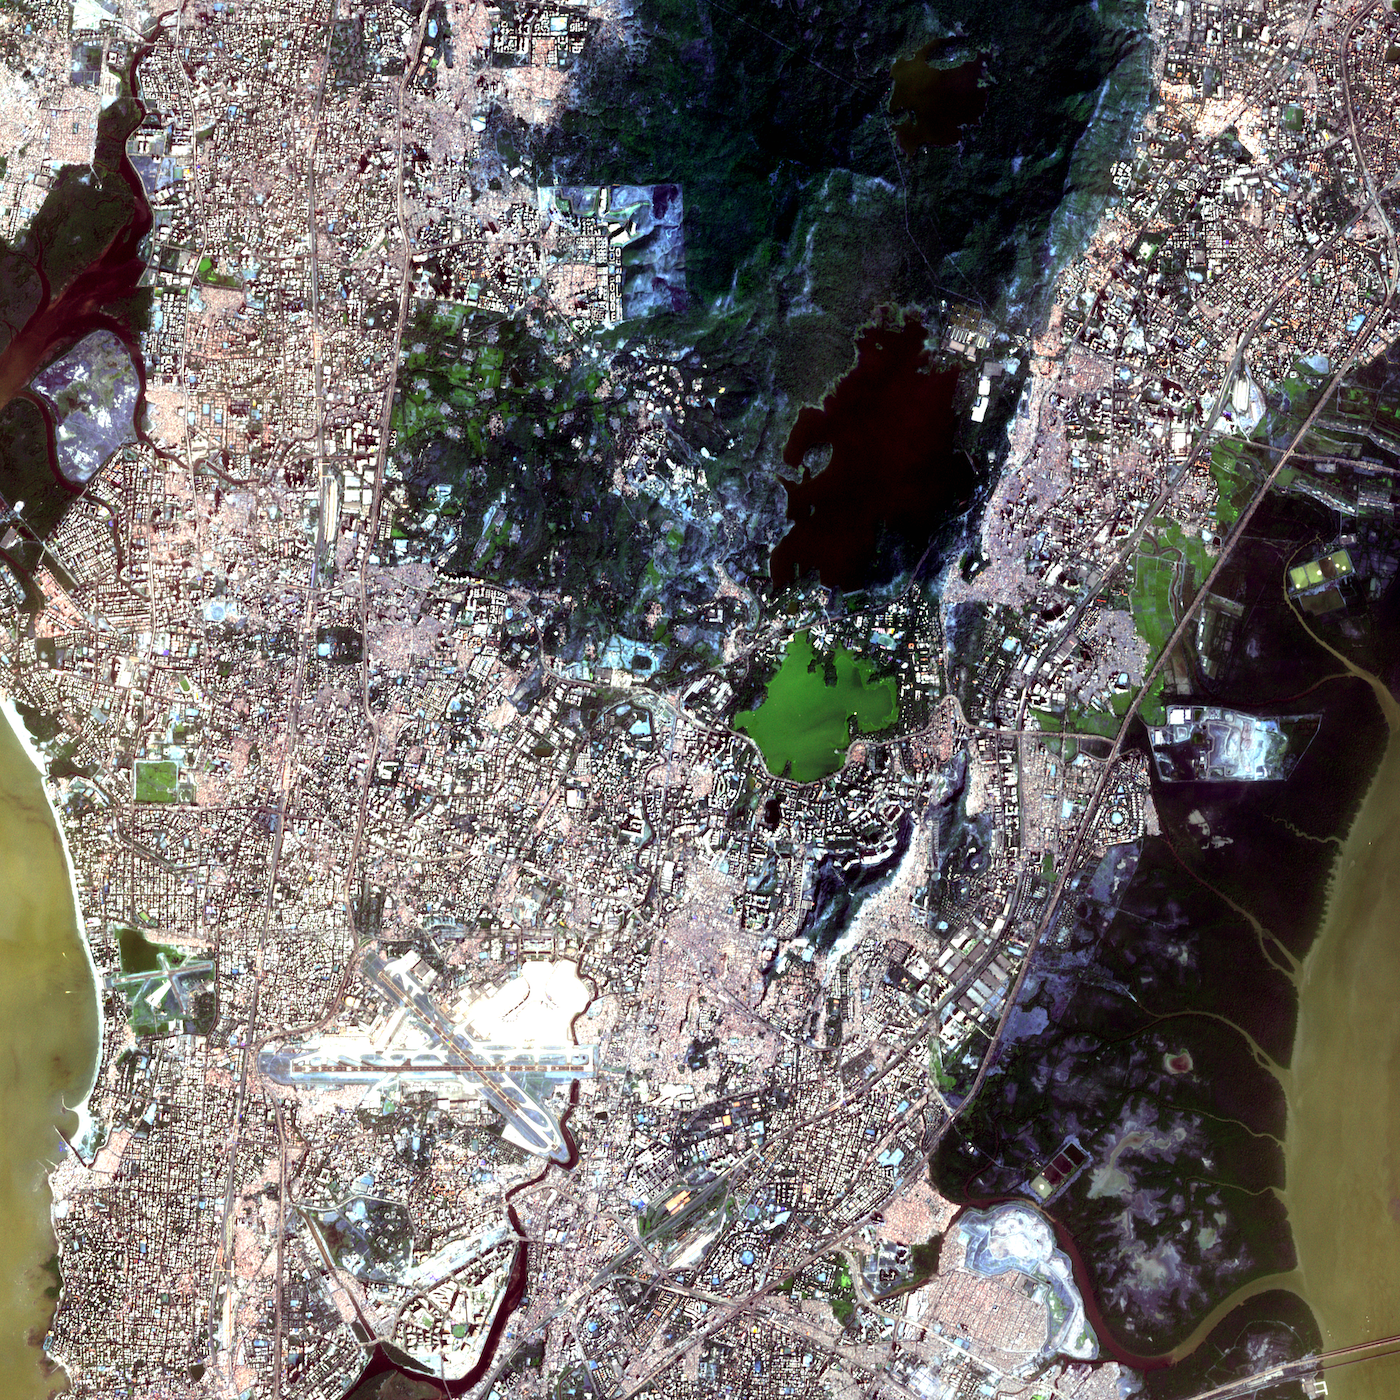
\includegraphics[width=\textwidth]{sat_image_run}
    \caption{}
  \end{subfigure}
  \caption[Predictions]{\textbf{(a)} Predictions using our model. \textbf{(b)} Predictions just using the road-detection model. \textbf{(c)} Image used to find predictions. Comparing the original road-detection model with the improved model.}
  \label{fig:run_merge_road_maps}
\end{figure}


\section{Cons}
One of the most noticeable drawbacks of using this model is the amount of time required to get the predictions. 

Another disadvantage is, the model is too much affected due to inaccuracies in the training dataset. If the road gets too thick, say, we take an image with a higher resolution, and run the model; we see that our model has several discontinuities in between. Refer (\cref{fig:cons_coverleaf}). This is mainly because of the noise which has effected the weights. This error can be reduced by training the model with more precise data. Another way to correct this error is to run the algorithm without super-resolution. This means we need to train the model again, this time without super-resolution.

\begin{figure}[h!]
  \centering
  \begin{subfigure}{0.3\textwidth}
    \includegraphics[width=\textwidth]{cons_coverleaf}
    \caption{}
  \end{subfigure}~
  \begin{subfigure}{0.3\textwidth}
    \includegraphics[width=\textwidth]{cons_road_coverleaf}
    \caption{}
  \end{subfigure}~
  \begin{subfigure}{0.3\textwidth}
    \includegraphics[width=\textwidth]{cons_road_coverleaf_sr}
    \caption{}
  \end{subfigure}
  \caption[Problem in predictions large roads]{\textbf{(a)} The image to apply the model on. \textbf{(b)} Road detection without applying super-resolution. \textbf{(c)} Road detection by out model. When a wide road is to be predicted, the noise takes over and our predictions go horribly wrong.}
  \label{fig:cons_coverleaf}
\end{figure}


Now that we have two predictions, one with super-resolution and without it, we merge them. First, we need to make them of the same resolutions. We do this by finding out the difference factor. Let us say the difference factor is $X$ on each side; we split the lower resolution image pixels into $X$ different pixels on both sides. Then we average the resultant images of the same resolution. For reference: look at \cref{fig:roads_in_confidence}

\begin{figure}[h!]
  \begin{subfigure}[b]{0.25\textwidth}
    \includegraphics[width=\textwidth]{roads_with_SR}
    \caption{}
  \end{subfigure}~
  \begin{subfigure}[b]{0.15\textwidth}
    \includegraphics[width=\textwidth]{roads_without_SR}
    \caption{}
  \end{subfigure}~
  \begin{subfigure}[b]{0.25\textwidth}
    \includegraphics[width=\textwidth]{roads_without_SR_zoomed}
    \caption{}
  \end{subfigure}~
  \begin{subfigure}[b]{0.25\textwidth}
    \includegraphics[width=\textwidth]{roads_with_confidence}
    \caption{}
  \end{subfigure}
  \caption[Finding likelihood of roads in predictions]{Merging roads found with \textbf{(a)} Predictions with SR. \textbf{(b)} Predictions without SR. \textbf{(c)} Upscaling of (b). \textbf{(d)} Final result by averaging (a) and (c). Black ones are definitely a road, grey ones having 0.5 probablity of being a road and least likely to find a road on the white pixel.}
  \label{fig:roads_in_confidence}
\end{figure}

\begin{sidewaysfigure}
  \centering
  \includegraphics[width=\textheight]{the_complete_picture}
  \caption{A figure summarising the complete process into one}
  \label{fig:the_complete_picture}
\end{sidewaysfigure}

% \chapter{Conclusions}
% \chapter{Scope of Improvements}
% https://towardsdatascience.com/road-segmentation-727fb41c51af
\pagebreak

\begin{appendices}
\chapter{Appendix}\label{chapt:appendix}
\section{code}
\end{appendices}
\normalem
\bibliographystyle{unsrtnat} 
%\bibliography{longnamesfirst,semicolon}
\bibliography{bibliography}
\addcontentsline{toc}{chapter}{\numberline{}References}

% % Adding a bibliography if citations are used in the report
% \bibliographystyle{plain}
% \bibliography{bibliography.bib}
% % Adds reference to the Bibliography in the ToC
% \addcontentsline{toc}{chapter}{\bibname}
% % \printbibliography

% [1]: Arin Basu. (April 16 2017). How to add footnotes https://medium.com/@arinbasu/you-can-use-footnotes-thus-babus%C2%B9-6c485c4eff1e

\pagebreak

% \chapter*{Appendix A: Resources}
% [\textit{Report the config files of the software used (i.e. SU2 \cite{economon2015su2} and the mesher). Also attach to this report an archive with the mesh files, solutions and the reference solution data (e.g. data points of a Cp plot ...)}]
% \section*{Mesh configuration files}
% \section*{SU2 configuration files}
% \section{Reference solution data}


\end{document}